%
% File acl2015.tex
%
% Contact: car@ir.hit.edu.cn, gdzhou@suda.edu.cn
%%
%% Based on the style files for ACL-2014, which were, in turn,
%% Based on the style files for ACL-2013, which were, in turn,
%% Based on the style files for ACL-2012, which were, in turn,
%% based on the style files for ACL-2011, which were, in turn, 
%% based on the style files for ACL-2010, which were, in turn, 
%% based on the style files for ACL-IJCNLP-2009, which were, in turn,
%% based on the style files for EACL-2009 and IJCNLP-2008...

%% Based on the style files for EACL 2006 by 
%%e.agirre@ehu.es or Sergi.Balari@uab.es
%% and that of ACL 08 by Joakim Nivre and Noah Smith

\documentclass[11pt]{article}
\usepackage{acl2015}
\usepackage{times}
\usepackage{url}
\usepackage{latexsym}
\usepackage{graphicx}
\usepackage[]{algorithm2e}
\usepackage{amssymb}
\usepackage{amsmath}
\usepackage[inline]{enumitem}
\usepackage{color}
\DeclareMathOperator{\eventcategory}{c}
\DeclareMathOperator{\corpus}{\mathcal{C}}
\DeclareMathOperator{\doc}{\mathnormal{d}}
\DeclareMathOperator{\sent}{\mathnormal{s}}
\DeclareMathOperator{\order}{\pi}
\DeclareMathOperator{\dtime}{\mathnormal{t}}
\DeclareMathOperator{\hour}{\mathnormal{h}}
\DeclareMathOperator{\hours}{\mathcal{H}}
\DeclareMathOperator{\Sim}{\mathbf{K}}
\DeclareMathOperator{\SMat}{\mathbf{X}}
\DeclareMathOperator{\Pref}{\boldsymbol{\pi}}
\DeclareMathOperator{\Exemp}{\mathnormal{Exemplars}}
\DeclareMathOperator{\Updates}{\mathnormal{Updates}}


\newcommand{\tsvec}[1]{\mathbf{#1}}
\newcommand{\tsveci}[2]{#1_{#2}}
\newcommand{\tsmat}[1]{\mathbf{#1}}
\newcommand{\tsmatij}[3]{#1_{#2#3}}

\newcommand{\query}[0]{q}
\newcommand{\stime}[0]{t_s}
\newcommand{\etime}[0]{t_e}

\newcommand{\features}[0]{\tsvec{x}}
\newcommand{\featuresi}[1]{\tsveci{x}{#1}}

\newcommand{\kernelMatrix}[0]{\tsmat{K}}
\newcommand{\kernelMatrixij}[2]{\tsmatij{K}{#1}{#2}}

\newcommand{\numfeatures}[0]{n}

\newcommand{\candidates}[0]{\mathcal{S}}
\newcommand{\numcandidates}[0]{|\candidates|}

\newcommand{\candidateSimMat}[0]{\tsmat{S}}
\newcommand{\candidateSimMatij}[2]{\tsmatij{S}{#1}{#2}}

\newcommand{\preferences}[0]{\tsvec{\pi}}
\newcommand{\fdadd}[1]{\textcolor{red}{#1}}
\newcommand{\fdcomment}[1]{\textbf{\textcolor{red}{[FD: #1]}}}
\newcommand{\ckcomment}[1]{\textbf{\textcolor{blue}{[CK: #1]}}}
\newcommand{\kmcomment}[1]{\textbf{\textcolor{green}{[KM: #1]}}}
%\setlength\titlebox{5cm}

% You can expand the titlebox if you need extra space
% to show all the authors. Please do not make the titlebox
% smaller than 5cm (the original size); we will check this
% in the camera-ready version and ask you to change it back.


\newenvironment{blockquote}{%
  \par%
  \medskip
  \leftskip=1em\rightskip=1em%
  \noindent\ignorespaces}{%
  \par\medskip}

\title{Unnamed Summarization Project}

%\author{First Author \\
%  Affiliation / Address line 1 \\
%  Affiliation / Address line 2 \\
%  Affiliation / Address line 3 \\
%  {\tt email@domain} \\\And
%  Second Author \\
%  Affiliation / Address line 1 \\
%  Affiliation / Address line 2 \\
%  Affiliation / Address line 3 \\
%  {\tt email@domain} \\}

\date{}

\begin{document}
\maketitle
\begin{abstract}
During crises such as natural disasters or other human tragedies, information
needs of both civilians and responders often require urgent, specialized
treatment.  
Monitoring and summarizing a text stream
during such an event remains a difficult problem. 
We present a system for update summarization which predicts the salience of 
sentences with respect to an event and then uses these
predictions to directly bias a clustering algorithm for sentence selection,
increasing the novelty of the updates. We use novel, disaster-specific features
for salience prediction, including geo-locations and language models
representing the language of disaster.
Our evaluation on a standard set of retrospective events using ROUGE shows 
that salience prediction provides a significant improvement over 
other approaches.

%The update summarization
%task refers to extracting short, sentence-length updates about a seed event
%from a stream of text data.
%Slow or ineffective information access can significantly impact the
%safety and health of individuals. 

%We evaluate our system on a standard set of retrospective events using
%the ROUGE automatic evaluation measures. 
%We
%demonstrate the effect of different feature groups, and the importance of
%salience prediction for update selection.

\end{abstract}

\section{Introduction}

\label{sec:introduction}

During crises, information is critical for first responders, crisis management
organizations, and those caught in the event. When the event is significant, 
as in the case of Hurricane Sandy, the amount of content produced by 
traditional news outlets, government agencies, relief organizations, and 
social media can vastly overwhelm those trying to monitor the situation. 
Crisis informatics \cite{palen2010vision} is dedicated to finding methods for 
sharing the right information in a timely fashion during such an event.
Research in this field has focused on human-in-the-loop approaches ranging 
from on the ground information gathering to crowdsourced reporting and 
disaster management \cite{starbird2013working}.


Multi-document summarization has the potential to assist the crisis 
informatics community. Automatic summarization could deliver relevant and 
salient information at regular intervals, even when human volunteers are 
unable to. Perhaps more importantly it could help filter out unnecessary and 
irrelevant detail when the volume of incoming information is large. While 
methods for identifying, tracking, and summarizing events from text based 
input have been explored extensively
\cite{allan1998topic,Filatova&Hatzivassiloglou.04a,Wang&al.11}, 
these experiments were not developed to handle streaming data from a
heterogeneous environment at web scale. These methods also rely heavily on 
redundancy which is suboptimal for time sensitive domains where there is a 
high cost in delaying information.


In this paper, we present an update summarization system to track events
across time. Our system predicts sentence salience in the context of a
large-scale event, such as a disaster, and integrates these predictions into
a clustering based multi-document summarization system. We demonstrate that 
combining salience with clustering produces more relevant summaries compared 
to baselines using clustering or relevance alone.  Our experiments suggest 
that this is because our system is better able to adapt to dynamic changes in 
input volume that adversely affect methods that use redundancy as a proxy for 
salience. 


In addition to the tight integration between clustering and salience
prediction, our approach also exploits knowledge about the event to determine
salience. Thus, salience represents both how typical a sentence is of the  
event
type (e.g., industrial accident, hurricane, riot) and whether it specifies 
information
about this particular event. 
Our feature representation includes a set of language models, one for each
event type, to measure the typicality of the sentence with regard to the 
current event, the distance of mentioned locations from the center of
the event, and the change in word frequencies over the time of the event.
While we evaluate these features in the domain of disasters, this approach is 
generally applicable to many update summarization tasks.


Our approach achieves a statistically significant improvement in ROUGE scores 
compared to multiple baselines. Additionally, we introduce novel methods for 
estimating the average information gain each update provides and how 
completely the update summary covers the event it is tracking; our system's 
updates contain more relevant information on average than the competing 
baselines.


The remainder of the paper is organized as follows. We begin with a review of 
related work in the information retrieval and multi-document summarization 
literature. Section~\ref{sec:methods} outlines the details of our salience 
and summarization models. Next we describe our data (Section~\ref{sec:data}) 
and experiments (Section~\ref{sec:exper}). Finally, we discuss our results 
(Section~\ref{sec:results}) and conclude the paper.


\section{Related Work}
\section{Related Work}
\label{sec:relatedwork}
A principal concern in extractive multi-document summarization is the
selection of salient sentences for inclusion in summary output
\cite{nenkova2012survey}.  This has often been approached as a ranking
problem.
%We broadly conceptualize this decision as either an intrinsic or extrinsic
%sentence evaluation process. Intrinsic approaches evaluate sentences
%individually, possibly by predicting the impact on summary quality using
%sentece level features. 
Sentences have been ranked by the average word probability, average tf-idf
score, and the number of topically related words (topic-signatures in the
summarization literature)
\cite{nenkova2005impact,hovy1998automated,lin2000automated}. The first two
statistics are easily computable from the input sentences, while the third
only requires an additional, generic background corpus.  Another ranking
approach, centroid summarization, involves creating an average bag of words
(BOW) vector, the centroid, from the input sentences and ranking sentences by
their similarity to the centroid \cite{radev2004centroid}.  Graph
\cite{erkan2004lexrank} and clustering
\cite{hatzivassiloglou2001simfinder,mckeown1999towards,siddharthan2004syntactic}
based approaches, on the other hand, make use of pair-wise similarity
comparisons amongst input sentences.  In these models, salient sentences are
more central to the input or cluster, respectively.

%identify salient regions of the input space while simultaneously coping with
%redundancy.  Graph-based algorithms have been used to rank sentences
%Clustering algorithms, e.g., are commonly used to exploit redundancy in
%input. Input sentences are clustered and summaries are generated by selecting
%the most representative sentence from each cluster.  Graph-based models have
%also been used for summarization.  E.g., the LexRank algorithm treats
%sentences as nodes in a graph, where edges are constructed by way of cosine
%similarity between sentence nodes; edges are either continuosly weighted by
%similarity or discrete, existing only when the similarity is above a
%threshold.  The PageRank algorithm is used on the graph to find the most
%important sentence nodes. In both clustering and graph-based approaches,
%sentence salience is largely determined by the pairwise relations between
%sentences.

Supervised learning has also been applied to this task. Model features are
usually derived from human generated summaries, and are non-lexical in nature
(e.g., sentence starting position, number of topic-signatures, number of
unique words, word frequencies). Seminal work in this area has employed naive
Bayes and logistic regression classifiers to identify sentences for summary
inclusion \cite{kupiec1995trainable,conroy2001using}. 

%\fdadd{
Several researchers have recognized the importance of summarization during
natural disasters.  Guo \textit{et al.} developed a system for detecting
novel, relevant, and comprehensive sentences immediately after a natural
disaster \cite{qi:temporal-summarization}.  The method uses a model of
sentence relevance and novelty in order to select appropriate updates.
Training data for regression targets is automatically generated from
retrospective Wikipedia data.  The system is evaluated on news documents
related to 197 natural and human disasters from 2009 to 2011 using variants of
Rouge modified to capture novelty, relevance, and comprehensiveness
\cite{lin2004rouge}.  Wang and Li present a clustering-based approach to
efficiency detect important updates during natural disasters
\cite{wang:update-summarization}.  The algorithm works by hierarchically
clustering sentences online, allowing the system to output a more expressive
narrative structure than Guo \textit{et al.}.  The method is evaluated on
official press releases related to Hurricane Wilma  in 2005 using Rouge score
between the system summary and a manually generated target summary.

\fdcomment{Glasgow temporal summarization system \cite{mccreadie:temporal-summarization}.}

\section{Method}
%In order to evaluate an update summarization system, we adopt the simulation-based approach used in the TREC Temporal Summarization (TS) Track.  We provide a brief overview of the problem.  Details on the formulation can be found in the track overview paper \cite{aslam2013trec}.  

Our update summarization system takes as input 
\begin{enumerate*}[label=\itshape\alph*\upshape)]
  \item a short query defining the event to be tracked (e.g. `Hurricane Sandy'), 
  \item an event category defining the type of event to be tracked (e.g. `hurricane'), 
  \item a stream of time-stamped documents %, $(\doc_0, \doc_1,\ldots,\doc_T)$,
  presented in temporal order, and \item an evaluation time period of interest.
    %  $(\stime,\etime)$.  
\end{enumerate*} 
While processing documents
throughout the time period of interest, the system outputs sentences
from these documents likely to be useful to query issuer.  We refer
to these selected sentences as \emph{updates}.

In order to measure the usefulness of a system's updates, we consider
the degree to which the system output reflects the different
aspects of an event.  Events are often composed of a variety of sub-events.  
For example, the Hurricane Sandy
event includes sub-events related to the storm making landfall,
the ensuing flooding, the many transportation issues, amongst many
others.  An ideal system would update the user about each of these
sub-events as they occur, with low latency.  In order to use
language consistent with previous literature, we refer to these
sub-events as the \emph{nuggets} associated with an event.  Nuggets are
defined as a fine-grained atomic sub-event associated with an event.  
We present several example nuggets associated with the Hurricane
Sandy event in Figure \ref{fig:nuggets}.  We describe how these 
nuggets are found in Section \ref{sec:data}.

% Updates should not only be relevant to the event but also salient,
% i.e. worthy of
% reporting.
% For most domains, updates also need to be
% timely and novel, i.e. users need to be informed of changes in the
% event as quickly as possible.
% Finally, in aggregate the updates must comprehensively summarize the
% event.

\begin{figure}
\setlength{\fboxsep}{10pt}
    \fbox{\parbox{6.9cm}{
        -- hurricane force wind warnings are in effect from Rhode Island Sound to Chincoteague Bay

        -- Obama declared an emergency in Maryland and signed an order authorized the Federal Emergency Management Agency to aid in disaster relief

        -- over 5000 commercial airline flights scheduled for October 28 and October 29 were cancelled
 }}
 \caption{Example nuggets from Hurricane Sandy.\label{fig:nuggets}}
\end{figure}


Throughout our treatment of our algorithm, the \emph{salience} 
of an update captures the degree to which it reflects an 
event's nuggets.  Assuming that we have a text representation 
of our nuggets, the salience of an update $u$  with respect to a set of nuggets $N$ is
defined as,
\begin{align}
\operatorname{salience}(u) = \operatorname{max}_{n \in N} 
\operatorname{sim}(u, n) \ref{eq:salience}
\end{align}
where $\operatorname{sim}(\cdot)$ is the semantic similarity such as
the cosine similarity of latent vectors associated with the update and 
nugget text \cite{?}. % We train
% a regression model to predict salience using features derived from
% the updates themselves
% and the document stream.



     % \ref{sec:methods}.  In our version of this problem, we assume that that
     % the system receives one batch of new sentence-segmented documents every
     % hour throughout the period of interest.
\subsection{Update Summarization}

Our system architecture follows a simple pipeline design where each
stage provides an additional level of processing or filtering of the input
sentences.
We begin with an empty update summary $U$.
At each hour we receive a new batch of sentences $b_t$ from the stream
and perform the following actions:
\begin{enumerate}
    \item predict the salience of sentences in $b_t$ (Section~\ref{sec:salpred}),
  \item select a set of exemplar sentences  in $b_t$ by combining clustering with 
      salience predictions (Section~\ref{sec:exsel}),
  \item add the most novel and salient exemplars to $U$ (Section~\ref{sec:upsel}).
\end{enumerate}

The resultant list of updates $U$ is our summary of the event.
% Step 2 uses the affinity propagation algorithm to incorporate the salience
% predictions from step 1. We refer to this summarization
% system as the \textbf{AP+Salience} model.


%\kmcomment{This was as best as I could do on this. These are the example
%    categories from the wikipedia page. However you refer in the language model
%    description to the event type earthquake which is more specific. Also, in
%    the TREC data you refer to event types that are specified in the metadata.
%So I'm wondering how many different categories you have and where they come
%from.}

%\fdcomment{include description of nuggets here.} 
%%\kmcomment{We should jointly
%    discuss what goes in data and what goes in problem definition. I have moved
%    event types here because I think knowing how many types and examples of
%    them would be helpful upfront. I think where nuggets and wikipedia pages go
%is questionable.}

%Figure \ref{alg:temporal-summarization} outlines our general update
%summarization algorithm.  At each hour, the system processes each input 
%sentence batch $S_t$.
%We predict the salience $P$ for all input sentences $s\in S_t$.
%Next, we cluster $S_t$ using the AP clustering algorithm, biased by $P$,
%obtaining a set of exemeplar sentences $E$. Finally we select a subset of $E$
%to be updates and add those to our set of summary updates $U$.
%
%\begin{algorithm}%[H]
% \KwData{ 
%     $S_{\stime}, S_{\stime+1},\ldots,S_{\etime} $ --- time ordered sentence
%     batches\\
% \KwResult{U --- a list of updates, i.e. the update summary} 
%}
% ~\\
% Initialize empty list $U$ of updates\\
%    \For{$t \gets \stime,\ldots,\etime $}{
%        $P \gets \operatorname{PredictSalience}(S_t)$\\
%        $E \gets \operatorname{APCluster}(P, S_t)$ \\
%        $U_t \gets \operatorname{SelectUpdates}(E,P,U)$\\
%        $U \gets U \cup U_t$
%}
% \caption{Temporal Summarization Algorithm}\label{alg:temporal-summarization}
%\end{algorithm}

\subsection{Salience Prediction}
\label{sec:salpred}

\subsubsection{Model}

When evaluating our summarization system
we do not have access to event nuggets. However, we can use the nuggets
in our training data to learn a model to predict salience for sentences
in new events.
For each event in our training data, we sample a set of sentences and  each 
sentence's salience is computed according to Equation \ref{eq:salience}.
This results in training set of set sentences and the target values 
(their salience) to predict.

In order to fit a regression model, the sentences are represented as feature
vectors (described in the next section).
We fit a Gaussian process (GP) regression model to this data.
\cite{rasmussen:gaussian-process-book}.  GP regressors are a
class of data-driven, non-parametric model generalizing the multi-variate
Gaussian to the infinite dimensional setting.  
%GP's are general
%and are state of the art for many regression tasks.  
GP's are non-parametric and rely on a covariance matrix $\kernelMatrix$, measuring the similarity between pairs of instances, in our 
case sentences.  In our experiments, we used a radial basis 
function (RBF) kernel.  
Our features fall naturally into five groups and we use a separate RBF kernel
for each, using the sum of each feature group kernel as the final input
to the GP model.

%include feature table
\begin{figure}[t!]
\begin{tabular}{| l |} 
\hline
\textbf{Basic Features}\\
$\cdot$ Sent. position (normalized by doc. length) \\
$\cdot$ Sent. length \\
$\cdot$ Ratio of punc./caps./lower/upper to \\
$\;\;$ other chars. \\
%$\cdot$ Ratio of caps. to non-caps. chars. \\
%$\cdot$ Ratio of lowercase to other chars. \\
%$\cdot$ Ratio of uppercase to other chars. \\
$\cdot$ \# of caps. words (normalized by \# of words)\\
$\cdot$ \# of Person, Location, Org., etc.\\
$\;\;$ (normalized by \# of words)\\
%$\;\;$ Ordinal, Percent, Money, Set, Misc  N.E. \\
\hline
\textbf{Query Features}\\
$\cdot$ \% of query words coverage/matches\\
$\cdot$ Total event-type synonyms/hypernyms/ \\
$\;\;$ hyponyms coverage/matches.\\
%$\cdot$ Total event-type synonyms/hypernyms/ \\
%$\;\;$ hyponyms matches.\\
\hline
\textbf{Language Model Features}\\
$\cdot$ Avg. token log probability (domain lang. \\
$\;\;$ model)\\
$\cdot$ Avg. token log probability (background \\
$\;\;$ lang. model)\\
\hline
\textbf{Geo-tag Features}\\
$\cdot$ Median document distance to nearest  \\
$\;\;$ location cluster (current hour/prev. hour).\\
%$\cdot$ Median document distance to nearest  \\
%$\;\;$ location clusters (previous hour).\\
$\cdot$ Distance of first location in doc. to nearest \\
$\;\;$ location cluster (current hour/prev. hour).\\
%$\cdot$ Distance of first location in doc. to nearest \\
%$\;\;$ location cluster (previous hour).\\
\hline
\textbf{Temporal Features}\\
$\cdot$ Avg. tf-idf at current time.\\
$\cdot$ Change in avg. tf-idf since previous hour \\
$\;\;$  (up to 24 hours).\\
$\cdot$ Time since query/event start.\\
\hline
\end{tabular}
\caption{Salience model features.}
\end{figure}


\subsubsection{Features}
We want our model to be predictive across different event instances so we avoid lexical features.  Instead, we extract a variety of features including language model scores, geographic relevance, and temporal relevance from each sentence.  

\paragraph{Basic Features}
%KM - Would be good to have quick justification of these features. I added a
%sentence. Feel free to edit or remove.

We employ several basic features that have been used previously in supervised models to rank sentence salience \cite{kupiec1995trainable,conroy2001using}. These include sentence length, the number of capitalized words normalized by sentence length, document position, number of named entities.  
The data stream comprises text extracted from raw html documents;
these features help to downweight sentences that are not actually article 
content (e.g. web page titles, links to other content) or
more heavily weight important sentences (e.g., that appear in
prominent positions such as paragraph initial or article initial).

\paragraph{Query Features}

Query features measure the relationship between the sentence and the event query and type.  These include the number of query words present in the sentence in addition to the number of event type synonyms, hypernyms, and hyponyms as found in WordNet \cite{miller1995wordnet}.  
For example, for event type \emph{earthquake},  we match sentence terms 
``quake'', ``temblor'', ``seism'', and ``aftershock''.

\paragraph{Language Model Features}\label{subsubsec:lm}
Language models allow us to measure the likelihood of a sentence having been 
produced from a particular source.  We consider two types of language model 
features.  The first model is estimated from a corpus of generic news 
articles \ckcomment{(we used the 199?-200? Associated Press and New York Times sections of the Gigaword corpus)}.  
This model is intended to assess the general writing quality (grammaticality, word usage) of an input sentence and helps our model to select sentences
written in the newswire style.  

The second model is estimated from text specific to our event types.  
For each event type we create a corpus of related documents using pages
and subcategories listed under a related Wikipedia category.
For example, the language model for event type `earthquake' is estimated 
from Wikipedia pages under the category \emph{Category:Earthquakes}.  

\fdcomment{stress here that this technique can be applied in situations beyond crisis; any situation where the
expected summary is similar to some previously seen target or some side information.}

These models are intended to detect sentences similar to those appearing in 
summaries of other events in the same category 
(e.g. most earthquake summaries are likely to include higher probability for 
ngrams including the token `magnitude').  

We use the SRILM toolkit to implement a 5-gram Kneser-Ney model for both
the background language and model and the event specific language models.
For each sentence we use the average token log probability under each model
as a feature.


%KM - Note: Someplace the exact list of event types should appear. Probably not
%here.
%KM - I note you have it in a later section but it is labeled as data you use
%to train language models and semantic similarity. I think it would be good to
%have up front in definition of task.


%For both models, we Finally, we extract the percentage of capitalized words,
%and sentence length as features. These last two features also help to
%identify sentences that are less likely to contain relevant content-- overly
%long and heavily capitalized sentences in our corpus were likely to be long
%strings of web-page headlines, section headers, and other irrelevant page
%structure. 

\paragraph{Geographic Relevance Features}
\fdcomment{need introduction here.  what are geographic features?}
There are two challenges to using geographic features. First we do not 
know where the event is and second most sentences do not contain references
to a location.
We address the first issue by extracting all locations from sentences at the
current hour and looking up their latitude and 
longitude using a publicly available geolocation service. 
\fdcomment{is this all documents in the bucket or the filtered set?  is it a biased sample?}
Since the document
stream contains documents that are at least somewhat relevant to the event,
we assume in aggregate the locations should give us a rough area of interest.
The locations are clustered (using affinity propagation and uniform salience)
\fdcomment{affinity propagation undefined}
and we treat the resulting cluster centers
as the event locations for the current time.

To address the second issue, 
we compute geographic relevance features for the document as a whole and all
sentences from that document receive the same feature value.
Using the locations in each document, we compute the median distance to the 
nearest event location. Because document position is a good indicator 
of importance we also compute the distance of the first mentioned
location to the nearest event location. Because some events can move, we also
compute these distances to event locations from the previous hour.



\paragraph{Temporal Relevance Features}
\fdcomment{motivate burstiness; explain what it is before using the expression.}
Our data consists of hourly crawls of online content and so we exploit the temporality of corpus by capturing the burstiness of a sentence, i.e.  the change in word frequency from one hour to the next.``Bursty'' sentences often indicate new and important data. 

We compute the IDF for each hour in our data stream. 
For each sentence, the average TFIDF for the current hour $t$ is taken as a 
feature. Additionally, we use the difference in average TFIDF from time $t$
to $t-i$ for $i = \{1, \ldots, 24\}$ to measure how the TFIDF scores for the 
sentence have changed over the last 24 hours. \fdcomment{unclear.  is it just changing the IDF part of the 
items in the average?}

The final temporal feature is the hours since the event started.
%difference 
%Using these IDF 
%calculations, the avg TFIDF is calculated for
%Let $D_t$ be the set of web pages at time $t$ and let $s = \{w_1,\ldots,w_n\}$ be a sentence from a page $d \in D_t$.  We calculate the 1-hour burstiness of sentence $s$ from document $d$ at hour $t$  as 
%\begin{align*}
%\operatorname{b}_1(s,d,t) = \frac{1}{|s|} \sum_{w \in s} \Bigg( &
%\operatorname{tf-idf}_t(w,d)  \\ & \left. - \frac{\sum_{d^\prime \in D_{t-1}:
%w \in d^\prime } \operatorname{tf-idf}_{t-1}(w,d^\prime)}{|\{d^\prime \in
%D_{t-1}: w \in d^\prime\}|} \right) \end{align*}

%where \begin{align*} \operatorname{tf-idf}_t(w,d) =&
%\log\left(1+\sum_{w^\prime \in d}1\{w=w^\prime\}  \right)\\ & \times
%\log\left(\frac{|D_t|}{1 + \sum_{d^\prime \in D_t}1\{w \in d^\prime\}}\right).
%\end{align*}

%[\textrm{Simpler explanation goes here}]
% 1\{w = w^\prime} %- \operatorname{avg-tf-idf}_{t_{i-1}}(w).
%\end{align*}


%We similarly find the sentence's 5-hour burstiness.  In addition to burstiness, we also include the sentence's average tf-idf and 


% Formally, let $p(f)$ be a distribution over functions where $f$ is any mapping
% of an input space $\mathcal{X}$ to the reals,
%
% $$f: \mathcal{X} \rightarrow \mathcal{R}.$$
% Let the random variable $\mathbf{f} = (f(x_1),\ldots,f(x_n) )$ be
%  an $n$-dimensional vector whose elements are evaluations of the function $f$
% at points $x_i \in \mathcal{X}$.
% We say $p(f)$ is a Gaussian process if for any finite subset
% $\{x_1,\ldots,x_n\} \subset \mathcal{X}$, the marginal distribution over
% that finite subset $p(\mathbf{f})$ has a multivariate Gaussian distribution.
% A GP is parameterized by a mean function $\mu(\mathbf{x})$ and a
% covariance function $K(x,x^\prime)$. Generally, the mean function is simply
% set to 0, leaving the distribution to be completely characterized by the
% kernel function on the data.
%
% In the regression setting, we typically have a response variable $y$ that
% is the sum of our model prediction  and
% some Gaussian noise, i.e. $y = f(x) + \epsilon$ with
% $\epsilon \sim \mathcal{N}(0, \sigma^2)$. When
% $f \sim \operatorname{GP}(\mathbf{0}, \mathbf{K})$, the
% two distributions
% of principal interest are the marginal likelihood
% $p(\mathbf{y}|\mathbf{X}) =
% \mathcal{N}(\mathbf{0},\mathbf{K} + \sigma^2\mathbf{I})$ and the predictive
% distribution,
%
% $$p(\mathbf{y_*}|\mathbf{x_*},\mathbf{X},\mathbf{y}) =
% \mathcal{N}(\boldsymbol{\mu}_*, \boldsymbol{\sigma}^2_*) $$
%
% where $\mathbf{x_*}$ is a new or unseen input, $\mathbf{y_*}$ our predicted
% response, and
% \begin{align*}
% \boldsymbol{\mu}_* & = \mathbf{K_*}(\mathbf{K} + \sigma^2\mathbf{I})^{-1}\mathbf{y} \\
% \boldsymbol{\sigma}^2_* &
% = \mathbf{K}_{**} - \mathbf{K}_*(\mathbf{K} + \sigma^2\mathbf{I})^{-1}
% \mathbf{K}_*^T + \sigma^2\\
% \end{align*}.
%
% Here $\mathbf{K}_* = K(\mathbf{x}_*, \mathbf{X})$, and
% $\mathbf{K}_{**} = K(\mathbf{x}_*, \mathbf{x}_*)$.
%
%

\subsection{Exemplar Selection}
\label{sec:exsel}

We combine the output of our salience prediction model with the affinity
propagation algorithm to identify a set of exemplar sentences 
for each input batch. 
Affinity propagation (AP) is a clustering algorithm
that identifies a subset of datapoints as exemplars and forms clusters
by assigning the remaining points to one of the exemplars. AP attempts to 
maximize the net similarity objective 
\[ \mathcal{S} = \sum_{i : i \neq e_i}^n \operatorname{sim}(i,e_i) 
+ \sum_{i : i = e_i}^n \operatorname{pref}(e_i)  \]
where $e_i$ is the exemplar of the $i$-th data point, and functions
$\operatorname{sim}$ and $\operatorname{salience}$ express the pairwise 
similarity
of data points and the apriori preference of a data point to be an exemplar
respectively. 
AP differs from other $k$-centers algorithms in that it simultaneously 
considers all data points as exemplars, making it less prone to finding
local optima as a result of poor initialization. Furthermore, the 
second term in $\mathcal{S}$ incorporates the individual importance of 
data points as candidate exemplars; most other clustering algorithms only make
use of the first term, i.e. the pairwise similarities between data points.
 
%There are very 
%few restrictions on the nature of the similarities and preferences
%other than that they be real-valued.

AP has several useful properties and interpretations. Chiefly, the number
of clusters $k$ is not a model hyper-parameter. Given that our task requires
clustering many batches of streaming data, searching for an optimal $k$ 
would be computationally prohibitive. With AP, $k$ is determined by the
similarities and preferences of the data. Generally lower preferences will
result in fewer clusters.  


%In our summarization system we use the output of our salience model as 
%the preferences, i.e.
%$\operatorname{salience}(s) = \operatorname{pref}(s)$; for the similarity 
%function we use semantic similarity. 
Recall that $\operatorname{salience}(s)$
is a prediction of the semantic similarity of $s$ to information about the 
event be summarized, i.e. the set of event nuggets.
Intuitively, when maximizing objective function $\mathcal{S}$, AP must balance
between best representing the input data and representing the most salient
input. Additionally, when the level of input is high but the salience
predictions are low, the preference term will guide AP toward a solution
with fewer clusters; vice-versa when input is very salient on average but
the volume of input is low. The adaptive nature of our model differentiates
our method from most out update summarization systems.




\subsection{Update Selection}
\label{sec:upsel}

\textbf{Salience Filter } To 
ensure that only the most salient updates are selected we apply a minimum
salience threshold;
after exemplar sentences have been identified, any exemplars whose salience is 
less than $\lambda_{sal}$ are removed from consideration. 

\textbf{Novelty Filter } Next,
to prevent adding updates that are redundant, we filter out exemplars
that are too similar to previous updates.
The exemplars are examined
sequencially in order of decreasing salience and  a similarity threshold 
is applied, where the exemplar is ignored if its
maximum semantic similarity to any previous updates in the summary is
greater than $\lambda_{sim}$.

Exemplars that pass these thresholds are added selected as updates and added
to the summary.






\section{Data}
\label{sec:data}
For the document stream, we use the news portion of the 2014 TREC KBA Stream 
Corpus \cite{frank2012building}. The documents from this corpus come from 
hourly crawls of the web covering October 2011 through February 2013. 


Our experiments also make use of the TREC Temporal Summarization (TS) Track
 data from 2013 and 2014 \cite{aslam2013trec}.  This data includes 25 events 
and event metadata (e.g., a user search query for the event, the event type, 
and event evaluation time frame). All events occurred during the time span of 
the TREC KBA Stream Corpus. For each event we create a stream of relevant 
documents by selecting only documents that contain the complete set of query 
words. 


Along with the metadata, NIST assessors constructed a set of ground truth 
nuggets for each event. Nuggets are brief and important text snippets that 
represent sub-events that should be conveyed by an ideal update summary. 
In order to accomplish this, for each event, assessors were provided with the
revision history of the Wikipedia page associated with the event. For example,
the revision history for the Wikipedia page for `Hurricane Sandy' will contain
text additions including those related to individual nuggets.  The assessment
task involves reviewing the Wikipedia revisions in the evaluation time frame 
and marking the text additions capturing a new, unique nugget.  More detail
on this process can be found in the track description \cite{aslam2013trec}.


\section{Experiments}
\label{sec:exper}
We evaluate our system on two metrics: ROUGE \cite{lin2004rouge}, an automatic
summarization method and an evaluation of system expected gain and 
comprehensiveness---metrics adapted from the TREC TS track 
\cite{aslam2013trec}.


\subsection{Training and Testing}


Of the 25 events in the TREC TS data, 24 are covered by the news portion of 
the TREC KBA Stream Corpus. From these 24, we set aside three events to use as
a development set. All system salience and similarity threshold parameters are
tuned on the development set to maximize ROUGE-2 F1 scores.


We train a salience model for each event using 1000 sentences randomly sampled
from the event's document stream. 


We perform a leave-one-out evaluation of each event. At test time, we predict 
a sentence's salience using the average predictions of the 23 other models.   


\subsection{ROUGE Evaluation}


ROUGE measures the ngram overlap between a model summary and an automatically 
generated system summary. Model summaries for each event were constructed by 
concatenating the event's nuggets. Generally, ROUGE evaluation assumes both 
model and system summaries are of a bounded length. Since our systems are 
summarizing events over a span of two weeks time, the total length of our 
system output is much longer than the model. To address this, for each 
system/event pair, we sample with replacement 1000 random summaries of length 
less than or equal to the model summary (truncating the last sentence when 
neccessary). The final ROUGE scores for the system are the average scores 
from these 1000 samples.


Because we are interested in system performance over time, we also evaluate 
systems at 12 hour intervals using the same regime as above. The model 
summaries in this case are retrospective, and this evaluation reveals how 
quickly systems can cover  information in the model.


\subsection{Expected Gain and Comprehensiveness}


NIST developed metrics for evaluating update summarization systems as part of 
the TREC TS track. We present results on two of these metrics, the expected 
gain and comprehensiveness.


\textbf{Expected Gain } We treat the event's nuggets as unique units of 
information. When a system adds an update to its summary, it is potentially 
adding some of this nugget information. It would be instructive to know how 
much unique and novel information each update is adding on average to the 
summary. To that end, we define
\[ \mathrm{\mathbb{E}[Gain]} = \frac{|S_n|}{|S|}
\] 
where $S$ is the set of system updates, $S_n$ is the set of nuggets contained 
in $S$, and $|\cdot|$ is the number of elements in the set. To compute the 
set $S_n$ we match each system update to 0 or more nuggets, where an update 
matches a nugget if their semantic similarity is above a threshold. $S_n$ 
results from the unique set of nuggets matched. Because an update can map to 
more than one nugget, it is possible to receive an expected gain greater 
than 1. An expected gain of 1 would indicate that every sentence was both 
relevant and contained a unique piece of information.


\textbf{Comprehensiveness } Additionally, we can use the nuggets to measure 
the completeness of an update summary. We define
\[ \mathrm{Comprehensiveness} = \frac{|S_n|}{|N|}\]
where $N$ is the set of event nuggets. A comprehensiveness of 1 indicates that
the summary has covered all nugget information for the event; the maximum
attainable comprehensiveness is 1.


Update-nugget matches are computed automatically; a match exists if the 
semantic similarity of the update/nugget pair is above a threshold. 
Determining an optimal threshold to count matches is difficult so we evaluate 
at threshold values ranging from .5 to 1, where values closer to 1 are more 
conservative estimates of performance. A manual inspection of matches suggests
that semantic similarity values around .7 produce reasonable matches.
The average semantic similarity of manual matches performed by NIST assessors 
was much lower at approximately .25, increasing our confidence in the 
automatic matches in the .5--1 range.


\subsection{Model Comparisons}


We refer to our complete model as \textsc{AP+Salience}.  We compare this model
against several variants and baselines intended to measure the contribution of
different components. All thresholds for all runs are tuned on the development
set.


\textbf{Affinity Propagation only (\textsc{AP}) } The purpose of this model 
is to 
directly measure the effect of integrating salience and clustering by 
providing a baseline that uses the identical clustering component, but without
the salience information. In this model, input sentences are \textit{apriori}
equally likely to be exemplars; the salience values are uniformly set as the 
median value of the  input similarity scores, as is commonly used in the 
\textsc{AP} 
literature \cite{frey2007clustering}. After clustering a sentence batch, the 
exemplars are examined in order of increasing time since event start and 
selected as updates if their maximum similarity to the previous updates is 
less than $\lambda_{sim}$, as in the novelty filtering stage of 
\textsc{AP+Salience}.


\textbf{Hierarchichal Agglomerative Clustering (HAC)} We provide another 
clustering baseline, single-linkage hierarchichal agglomerative clustering.
We include this baseline to show that \textsc{AP+Salience} is not just an 
improvement
over \textsc{AP} but centrality driven methods in general. \textsc{HAC} was 
chosen over other 
clustering approaches because the number of clusters is not an explicit 
hyper-parameter. To produce flat clusters from the hierarchical clustering, we
flatten the \textsc{HAC} dendrogram using the cophenetic distance criteria, 
i.e. 
observations in each flat cluster have no greater a cophenetic distance than a
threshold. Cluster centers are determined to be the sentence with highest 
cosine similariy to the flat cluster mean. Cluster centers are examined in 
time order and are added to the summary if their similarity to previous 
updates is below a similarity threshold $\lambda_{sim}$ as is done in the 
\textsc{AP} model.


\textbf{Rank by Salience (RS)} 
We also isolate the impact of our salience model in order to demonstrate 
that the fusion of clustering and salience prediction improves over
predicting salience alone. In this model we predict the salience of sentences 
as in step 1 for \textsc{AP+Salience}. We omit the clustering phase (step 2).
Updates are selected identically to step 3 of \textsc{AP+Salience}, 
proceeding in order
of decreasing salience, selecting updates that are above a salience 
threshold $\lambda_{sal}$ and below a similarity threshold $\lambda_{sim}$
with respect to the previously selected updates.


\section{Results}
\label{sec:results}

\subsection{ROUGE}
\begin{table}[h]
\centering
% centering table
\begin{tabular}{l c c c}
% creating 10 columns
\multicolumn{4}{c}{ROUGE-1}\\
\hline
\hline
% inserting double-line
$\mathrm{System}$ & $\mathrm{Recall}$ & $\mathrm{Prec.}$ & $\mathrm{F}_1$\\
[0.5ex]
\hline
AP+Salience & $0.282$ & $0.344$ & $0.306$ \\
AP          & $0.245$ & $0.285$ & $0.263$ \\
RS          & $0.230$ & $0.271$ & $0.247$ \\
HAC         & $0.169$ & $0.230$ & $0.186$ \\
\hline % inserts single-line
\end{tabular}
~\\[1ex]
~\\
\begin{tabular}{l c c c}
% creating 10 columns
\multicolumn{4}{c}{ROUGE-2}\\
\hline
\hline
% inserting double-line
$\mathrm{System}$ & $\mathrm{Recall}$ & $\mathrm{Prec.}$ & $\mathrm{F}_1$\\[0.5ex]
\hline
AP+Salience & $0.045$ & $0.056$ & $0.049$ \\
AP          & $0.033$ & $0.038$ & $0.035$ \\
RS          & $0.031$ & $0.037$ & $0.034$ \\
HAC         & $0.017$ & $0.024$ & $0.019$ \\
\hline % inserts single-line
\end{tabular}
~\\[1ex]
~\\
\begin{tabular}{l c c c}
% creating 10 columns
\multicolumn{4}{c}{ROUGE-L}\\
\hline
\hline
% inserting double-line
$\mathrm{System}$ & $\mathrm{Recall}$ & $\mathrm{Prec.}$ & $\mathrm{F}_1$\\[0.5ex]
\hline
AP+Salience & $0.275$ & $0.336$ & $0.299$ \\
AP          & $0.241$ & $0.280$ & $0.258$ \\
RS          & $0.225$ & $0.265$ & $0.242$ \\
HAC         & $0.166$ & $0.225$ & $0.182$ \\
\hline % inserts single-line
\end{tabular}


\caption{System ROUGE performance.} % title name of the table
\label{tab:rouge}
\end{table}






Table~\ref{tab:rouge} shows our results for system output samples against the full summary of nuggets using ROUGE. 
%shows our results for the evaluation using ROUGE. 
%AP+Salience shows improvement on ngram precision and recall over the 
%baselines. 
This improvement is statistically significant for all ngram
precision, recall, and F-measures
at the $\alpha = .01$ level
using the Wilcoxon signed-rank test. 

\begin{figure}
    \includegraphics[]{rouge-time.eps}
\caption{System ROUGE-1 performance over time.}
\label{fig:trouge}
\vspace{-14pt}
\end{figure}


AP+Salience maintains its performance above the baselines over time as well. Figure~\ref{fig:trouge}
shows the ROUGE-1 scores over time. 
We show the difference in unigram precision (bigram precision is not shown but it follows
similar curve).
Within the initial days of the event, AP+Salience is able to take the lead over the over 
systems in ngram precision. 
The AP+Salience model is better able to find salient updates
earlier on; for the disaster domain, this is an especially important quality of the model. 

Moreover, the AP+Salience's recall is not diminished by the high precision and remains competitive with AP.
Over time AP+Salience's recall also begins to pull away, while the other models start to suffer
from topic drift.


\subsection{Expected Gain and Comprehensiveness}
\begin{figure}
  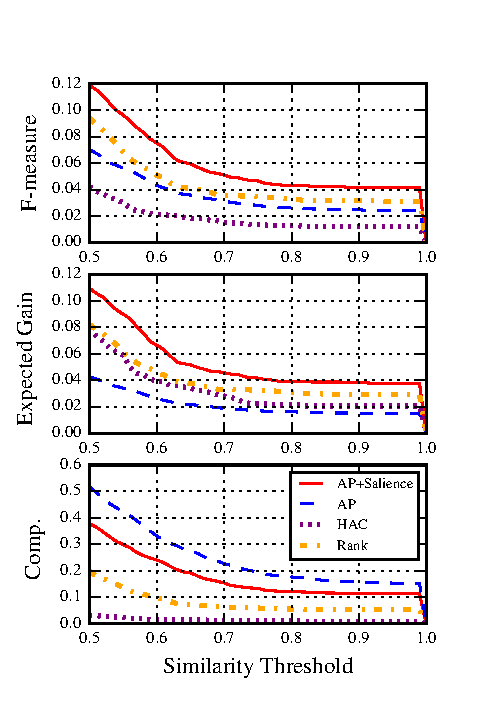
\includegraphics[]{nuggets-metrics.eps}
\caption{Expected Gain and Comprehensiveness performance.}
\label{fig:nperf}
\vspace{-12pt}
\end{figure}

Figure~\ref{fig:nperf} shows the expected gain across a range of 
similarity thresholds, where thresholds closer to 1 are more conservative
estimates. The ranking of the systems remains constant across the 
sweep with 
AP+Salience beating all baseline systems.
Predicting salience in general is helpful for keeping a summary on topic as
the RS approach out performs the clustering only approaches
on expected gain.

When looking at the comprehensiveness of the summaries AP outperforms
 AP+Salience. The compromise encoded in the AP+Salience objective
function, between being representitive and being salient, is seen clearly here
where the performance of the AP+Salience methods is lower bounded by 
the salience focused RS
system and upper bounded by the clustering only AP system.
Overall, AP+Salience achieves the best balance of these two metrics.



\subsection{Feature Ablation}
\begin{table}[h]
\centering
% centering table
\begin{tabular}{l c c c}
% creating 10 columns
\multicolumn{4}{c}{ROUGE-1}\\
\hline
\hline
% inserting double-line
$\mathrm{System}$ & $\mathrm{Recall}$ & $\mathrm{Prec.}$ & $\mathrm{F}_1$\\
[0.5ex]
\hline
Full System & $0.282$ & $0.344$ & $0.306$ \\
No Basic    & $0.263$ & $0.380^\dagger$ & $0.294$ \\
No LM       & $0.223^\dagger$ & $0.361$ & $0.254^\dagger$ \\
No Time  & $0.297^\dagger$ & $0.367^{\dagger\dagger}$ & $0.322^\dagger$ \\ 
No Geo   & $0.232^{\dagger\dagger}$ & $0.381$ & $0.265^\dagger$ \\  
No Query & $0.251$ & $0.377$ & $0.280$ \\ 
\hline % inserts single-line
\end{tabular}
~\\[1ex]
~\\
\begin{tabular}{l c c c}
% creating 10 columns
\multicolumn{4}{c}{ROUGE-2}\\
\hline
\hline
% inserting double-line
$\mathrm{System}$ & $\mathrm{Recall}$ & $\mathrm{Prec.}$ & $\mathrm{F}_1$\\[0.5ex]
\hline
Full System & $0.045$ & $0.056$ & $0.049$ \\
No Basic    & $0.046$ & $0.068^{\dagger\dagger}$ & $0.051^\dagger$ \\
No LM       & $0.033^\dagger$ & $0.056$ & $0.038^\dagger$ \\
No Time  & $0.052^{\dagger\dagger}$ & $0.064^{\dagger\dagger}$ & $0.056^{\dagger\dagger}$ \\
No Geo   & $0.037^\dagger$ & $0.065$ & $0.042$ \\
No Query & $0.043$ & $0.068^\dagger$ & $0.048$ \\
\hline % inserts single-line
\end{tabular}
\caption{Feature ablation ROUGE performance. 
    $\dagger$ indicates statistically significant difference from 
full model at the $\alpha=.05$ level.
    $\dagger\dagger$ indicates statistically significant difference from 
full model at the $\alpha=.01$ level.
    } % title name of the table
\label{tab:farouge}
\end{table}








Table~\ref{tab:farouge} shows the results of our feature ablation
tests. Removing the language models yields a statistically 
significant drop in both ngram recall and F-measure. 
Interestingly, removing the basic features leads to an
increase in both unigram and bigram precision; in the bigram
case this is enough to cause a statistically significant increase
in F-measure over the full model. In other words, the generic features
actually lead to an inferior model when we can incorporate more appropriate
domain specific features.
%This result mirrors Sparck Jones' claim that summarization should be in service of a purpose~\cite{?}.

Removing the language model and geographic relevance features leads to a
statistically significant drop in ROUGE-1 F1 scores. Unfortunately,
this is not the case for the temporal relevance features. We surmise that
these features are too strongly correlated with each other, 
i.e. the differences in TFIDF between hours are definitely not IID variables. 






\section{Conclusion}
In this paper, we have presented an update summarization system for the 
disaster domain, and demonstrated improved system performance by integrating 
sentence salience with clustering.


We also have shown that features specifically targeted to the domain of 
disaster yield better summaries. We developed novel features that capture the 
language typical of different event types and that identify sentences specific
to the particular disaster based on location.


In the future we would like to explore the application of the 
\textsc{AP+Salience}
model and features to a wider class of events. 


% include your own bib file like this:
\bibliographystyle{acl} 
\bibliography{cites}

% \begin{thebibliography}{}
%
% \bibitem[\protect\citename{Aho and Ullman}1972]{Aho:72} Alfred~V. Aho and
%     Jeffrey~D. Ullman.  \newblock 1972.  \newblock {\em The Theory of Parsing,
%     Translation and Compiling}, volume~1.  \newblock Prentice-{Hall}, Englewood
%     Cliffs, NJ.
%
% \bibitem[\protect\citename{{American Psychological Association}}1983]{APA:83}
%     {American Psychological Association}.  \newblock 1983.  \newblock {\em
%     Publications Manual}.  \newblock American Psychological Association,
%     Washington, DC.
%
% \bibitem[\protect\citename{{Association for Computing Machinery}}1983]{ACM:83}
%     {Association for Computing Machinery}.  \newblock 1983.  \newblock {\em
%     Computing Reviews}, 24(11):503--512.
%
% \bibitem[\protect\citename{Chandra \bgroup et al.\egroup }1981]{Chandra:81}
%     Ashok~K. Chandra, Dexter~C. Kozen, and Larry~J. Stockmeyer.  \newblock
%     1981.  \newblock Alternation.  \newblock {\em Journal of the Association
%     for Computing Machinery}, 28(1):114--133.
%
% \bibitem[\protect\citename{Gusfield}1997]{Gusfield:97} Dan Gusfield.  \newblock
%     1997.  \newblock {\em Algorithms on Strings, Trees and Sequences}.
%     \newblock Cambridge University Press, Cambridge, UK.
%
% \end{thebibliography}
%
\end{document}
